\scanpage{12}
\mspage{1}
\margin{23.12.83}

Structure sur l'ens des positions relatives $P=\operatorname{PR}(\underline\Sigma)$ d'un syst. $\underline\Sigma=(X,\Sigma)$ de pseudodroites.

a) Relations de spécialisation $D\longrightarrow D'$ (ou de générisation en sens inverse). À vrai dire, on a un ensemble $\widetilde P$ de ``flèches de spécialisation'' en paires $(D,T)$, où $D$ est dans $\operatorname{PR}$. et $T$ est un ``triangle de spécialisation'' pour $D$ i.e.
\deleted{c'est-à-dire}

\figure{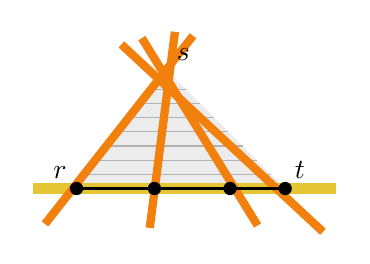
\begin{tikzpicture}[x=1cm,y=1cm]
\fill[gray!15] (0,0)--(1.15,1.5)--(2.65,0)--cycle;
\foreach \y in {.18,.36,.54,.72,.90,1.08,1.26}{\draw[gray!60,thin] ({.7667*\y},\y)--({2.65-\y},\y);}
\draw[yellow!55!brown,line width=4pt] (-.55,0)--(3.3,0);
\draw[orange!80!brown,line width=3pt] (-.4,-.45)--(1.48,1.94);
\draw[orange!80!brown,line width=3pt] (.93,-.5)--(1.25,1.99);
\draw[orange!80!brown,line width=3pt] (2.30,-.47)--(.83,1.91);
\draw[orange!80!brown,line width=3pt] (3.13,-.55)--(.57,1.83);
\draw[thick] (0,0)--(2.65,0);
\foreach \x in {0,.99,1.95,2.65}{\fill (\x,0) circle(2.4pt);}
\node[above right] at (1.15,1.5){$s$};\node[above left] at (0,0){$r$};\node[above right] at (2.65,0){$t$};
\end{tikzpicture}}

\deleted{\unsure{un sous-ens.} de $\nu\geq1$ sur $D$, \deleted{non réduites à un sommet de $\Sigma$, formant} un arc sur $\widetilde D$ (le rev. des \unsure{vis} de $D$, avec sa structure polygonale) et dont les $\nu+1$ sommets s'identifient aux \unsure{$\nu$-arêtes orientations} de $\widetilde D$) \deleted{\unsure{correspondant|correspondent} à $\nu+1$}\inserted{sont \unsure{non-sommets de}} $\Sigma$, et correspondent à des $D_i\in\Sigma$ que se rencontrent en un $=$ point $s$ \uline{d'ordre exactement} $\nu+1$, et sans sommet de $\Sigma$ dans le triangle $s,r,t$ \unsure{ni à l'intérieur, sauf} $s\ldots$}

[On exclut le cas où $\Sigma$ est trivial, qu'il est mieux traiter à part.] On a une application
\diagram{\begin{tikzcd}[ampersand replacement=\&]\widetilde P\arrow[r,"{(\text{source,but})}"]\&P\times P\end{tikzcd}}
qui associe à $(D,T)$ le couple $(D,D')$, où $D'$ est ``déduit de $D$ par balayage-spécialisation de $D$ au dessus de $T$''. Cette application est-elle injective? Quand on connaît $(D,D')$, on connaît aussi $s$ (qui est l'unique sommet de $\Sigma$ qui est dans $D'$, non dans $D$) donc aussi l'ens \deleted{des extrémités} des \inserted{$\nu+1$} sommets de $\Sigma\cup\{D\}$ qui sont inclus dans le triangle $T$ --- savoir les sommets communs à $D$ et aux $\nu+1$ éléments de $\Sigma$ passant par $s$. D'autre part, on voit qu'aucune de ces ps. droites (en tant que p. dr. de \deleted{$\unsure{\Sigma}$} $\Sigma'=\Sigma\cup\{D\}$) n'est un bigone, \deleted{ce qui} (sinon $\Sigma$ serait trivial de centre $s$) ce qui implique que les arêtes \deleted{joignant}\inserted{contenues} dans $T$ qui joignent $s$ aux $2$ sommets \deleted{\unsure{con.}} envisagés sur $D$, \unsure{sont ainsi uniques} \deleted{\unsure{d'autre p.}} \unsure{(les \unsure{vis|vts} de $\Sigma$ que sur $D$!)} \unsure{au moins un autre sommet que ceux-là}, ce qui implique que l'aire qu'ils \unsure{cernent} est également déterminée --- bref, $\widetilde P\to P\times P$ est bien injectif. On trouve donc un \uline{\unsure{graphe}}\inserted{\uline{strict orienté}} \unsure{simple} $P$ comme ens des sommets, $\widetilde P$ comme ens. d'arêtes, ch. que arête étant orientée \deleted{\unsure{d'un sens}}\inserted{(i.e. munie} d'une origine privilégiée).

\margin{\uline{NB} on a tjs $D\ne D'$, car $D'\cap S=(D\cap S)\cup\{s\}$}

Soit, pour $D\in P$, $\operatorname{Sp}_0(D)$ l'ens de ses spécialisations \inserted{(immédiates) ou ``successeurs''}, \deleted{et $\operatorname{Gen}(D)$ l'ens de ses} qui correspond à l'ens des triangles de spécialisation \unsure{formés|\deleted{formés}} pour $D$. Soit de $=$ $\operatorname{Gen}_0(D)$ l'ens de ses générisations (immédiates), qui correspond à l'ens des couples $(s,\widetilde{\unsure{\varphi|\xi}})$, où $s\in D\cap S$, et $\widetilde{\unsure{\varphi|\xi}}$ est une or. de $D$ en $s$ i.e. un pt de $\widetilde D$ sur $s$.

\margin{11}
